\chapter{XUV Light Source Design and Apparatus Performance}

\section{The need for high XUV flux in ATAS experiments}

\section{Harmonic Gas Sources}

\subsection{free expansion gas jet nozzle}

\subsection{low pressure cell}

\subsection{high pressure cell}
\label{sec:HPC}

\subsection{amsterdam pulsed piezoelectric valve}

\section{characterization of XUV source}

\subsection{knife edge measurements at XUV focus}

\begin{figure}
	\centering
	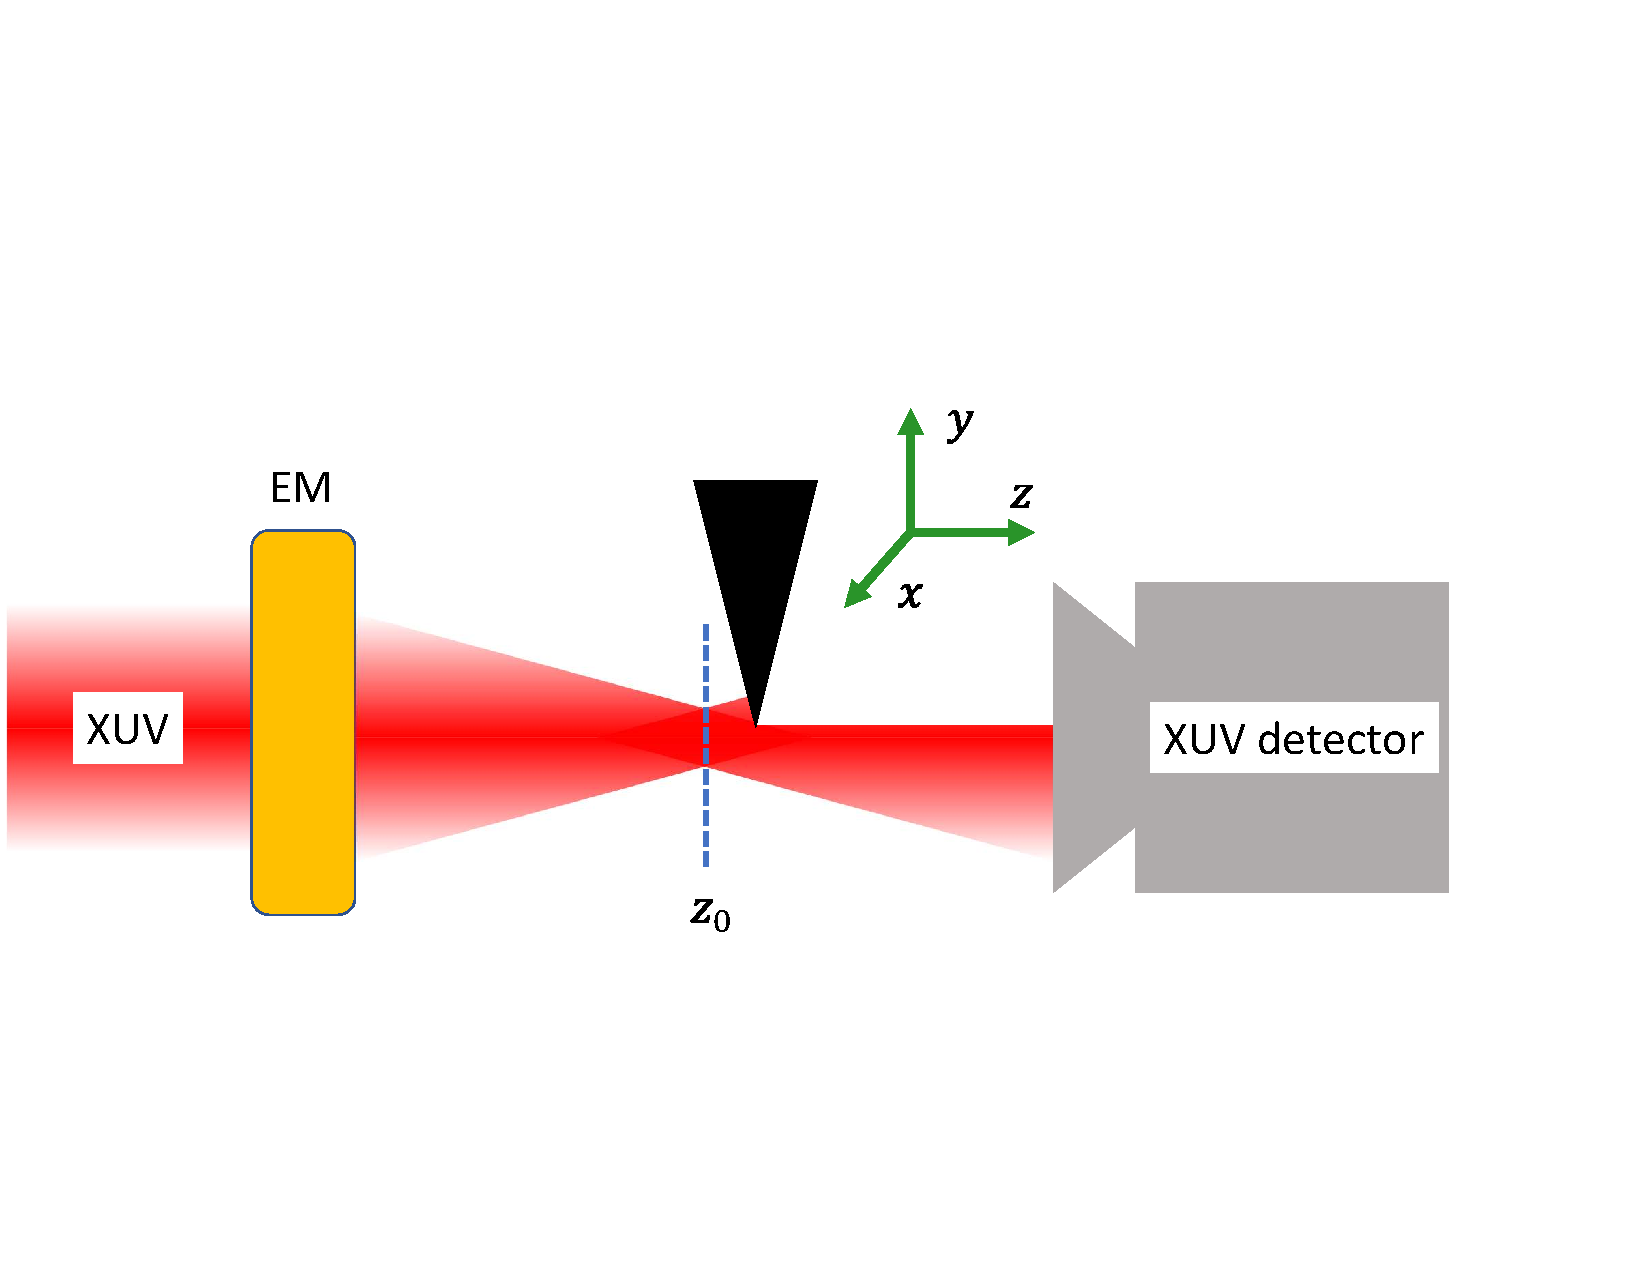
\includegraphics[width=0.75\textwidth]{figures/chap3/knife_edge_cartoon.pdf}
	\caption{Schematic of XUV knife edge measurement. EM: ellipsoidal mirror, $z_0$: XUV focal plane.}
	\label{fig:knife_edge_cartoon}
\end{figure}

\begin{figure}
	\centering
	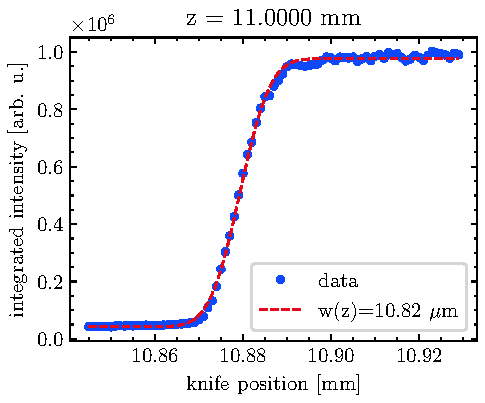
\includegraphics[width=0.75\textwidth]{figures/chap3/XUV_focus_knife_edge.pdf}
	\caption{A typical XUV knife edge measurement near the focal plane. The sample motor position is $k=11.0000$ mm. A fit to equation \cref{eqn:knife_edge} yields a beam waist of 10.82 $\mu$m at this position.}
	\label{fig:XUV_focus_knife_edge}
	% dataset: C:\testdata\2019_08_23\knife\11.0000
	% python file: \Python Scripts\Spectrometer\test\knife_edge.py
\end{figure}

\begin{figure}
	\centering
	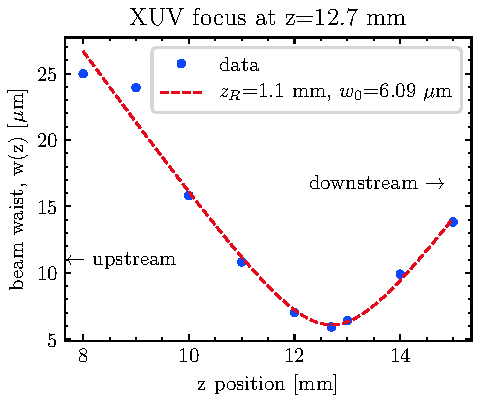
\includegraphics[width=0.75\textwidth]{figures/chap3/XUV_waist_vs_k.pdf}
	\caption{Evolution of XUV beam waist as a function of propagation direction, $z$. The Rayleigh range $z_R$ and beam waist $w_0$ are extracted from the fit to \cref{eqn:beam_waist_evolution}.}
	\label{fig:XUV_waist_vs_k}
	% question: what is $M^2$ value of the XUV?. or, does w0 and zR change with XUV wavelength?
	% dataset: C:\testdata\2019_08_23\knife\11.0000
	% python file: \Python Scripts\Spectrometer\test\knife_edge.py
\end{figure}

We characterize the XUV focus in the target chamber by performing knife edge measurements at different $k$-positions, as depicted in \cref{fig:knife_edge_cartoon}. We use the interior angled edge of the Si frame on a broken sample heterostructure as a knife edge (see \cref{fig:Sample_Geometry}). This frame makes an excellent knife edge as it has a very well-defined geometry and fits in the sample holder. Recalling Gaussian optics, the assumed profile of the XUV beam is:
\begin{equation}
I(x,y,z) = I_0 \left( \frac{w_0}{w(z)} \right)^2 \exp \left( - 2 ((x-x_0)^2 + (y-y_0)^2) /  w(z)^2 \right),
\end{equation}
using the coordinate system defined in \cref{fig:knife_edge_cartoon}. The XUV focus is at position $(x_0,y_0,z_0)$. The beam waist $w(z)$ will evolve as:
\begin{equation}
w(z) = w_0 \sqrt{ 1 + \left( \frac{z-z_0}{z_R} \right)^2 },
\label{eqn:beam_waist_evolution}
\end{equation}
where $z_R$ is the Rayleigh range. If we use the knife edge to block the transmission as depicted in \cref{fig:knife_edge_cartoon}, then the transmitted power will be:
\begin{equation}
P(x, z) = P_0 + \frac{P_{max}}{2} \left( 1 - \erf \left( \frac{\sqrt{2}(x-x_0)}{w(z)} \right) \right),
\label{eqn:knife_edge}
\end{equation}
where $x$ is the insertion of the knife in the beam, $z$ represents the location of the knife plane in the propagation direction, and $\erf$ is the error function.

A typical knife edge measurement is shown \cref{fig:XUV_focus_knife_edge}. In this measurement, the knife edge is translated across the XUV spot in 1 $\mu$m steps until the XUV light is completely blocked. A 2D spectrum is saved at each knife edge position. Each image is background subtracted, normalized and summed (integrating over all divergences and wavelengths), which yields the XUV flux as a function of knife position. The resulting curve is fit to \cref{eqn:knife_edge} and the beam waist $w(z)$ is extracted for this $z$-position.

The knife edge measurement is repeated at different $z$-positions until enough data has been acquired to determine the focal plane. The evolution of the XUV beam waist is shown in \cref{fig:XUV_waist_vs_k}. In this figure, the beam waist has been fit to \cref{eqn:beam_waist_evolution} to determine the focal plane $z_0$, the Rayleigh range $z_R$ and the beam waist $w_0$. In both figures, a reasonably good fit is obtained, indicating that the XUV light has a Gaussian spatial profile near the focus.


\subsection{harmonic yield stability}

\subsection{XYV spectra optimized for various HHG conditions}

\subsection{Measured Transmission of Metallic Filters}

\subsection{Ground State Measurements of Condensed Matter Samples}

\section{characterization of interferometric stability}

\section{MCP response}

scaling of yield and noise with respect to MCP voltage